\begin{enumerate}
    \item \alert{実空間}で8-Chain Model で初期構造を作成。
        \begin{itemize}
            % \item \alert{実空間}で8-Chain Model で初期構造を作成。
            % \item 所望の分岐数に\alert{ランダム}に選択した\alert{結合を除去}
            \item 除去したジオメトリーに対応した\alert{トポロジーモデル}
        \end{itemize}
    \item トポロジー空間でランダム性の導入
        \begin{itemize}
            % \item ラプラシアン行列で全体の接続性を確認しながら、
            \item \alert{エッジ交換}して、ネットワーク構造にランダムな接続性を導入
        \end{itemize}	
    \item 対応する\alert{実空間でのネットワーク初期構造}を作成
    \item \alert{ストランド長がホモポリマーに対応}するように多重度設定して、\\ \alert{Slow Push Off により初期構造を緩和}
\end{enumerate}

\vspace{-1mm}
\begin{columns}[T, onlytextwidth]
    \column{.33\linewidth}
        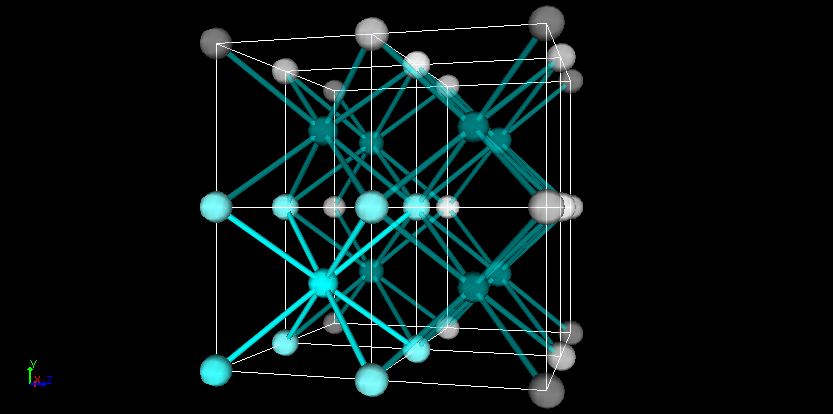
\includegraphics[width=\textwidth]{8_per.png}
    \column{.33\linewidth}
        \vspace{-5mm}
        \begin{center}
            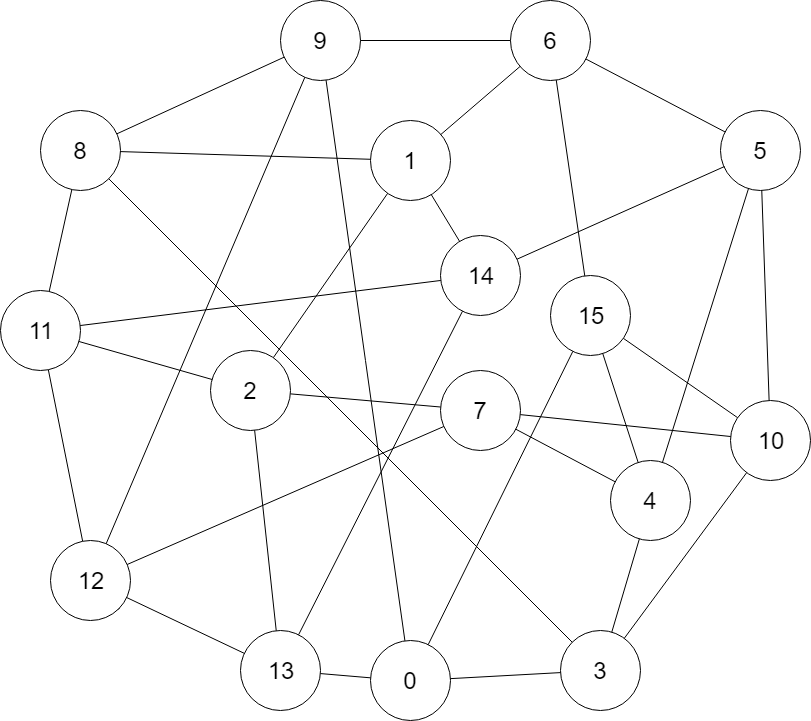
\includegraphics[width=.6\textwidth]{Network.png}
        \end{center}
    \column{.33\linewidth}
        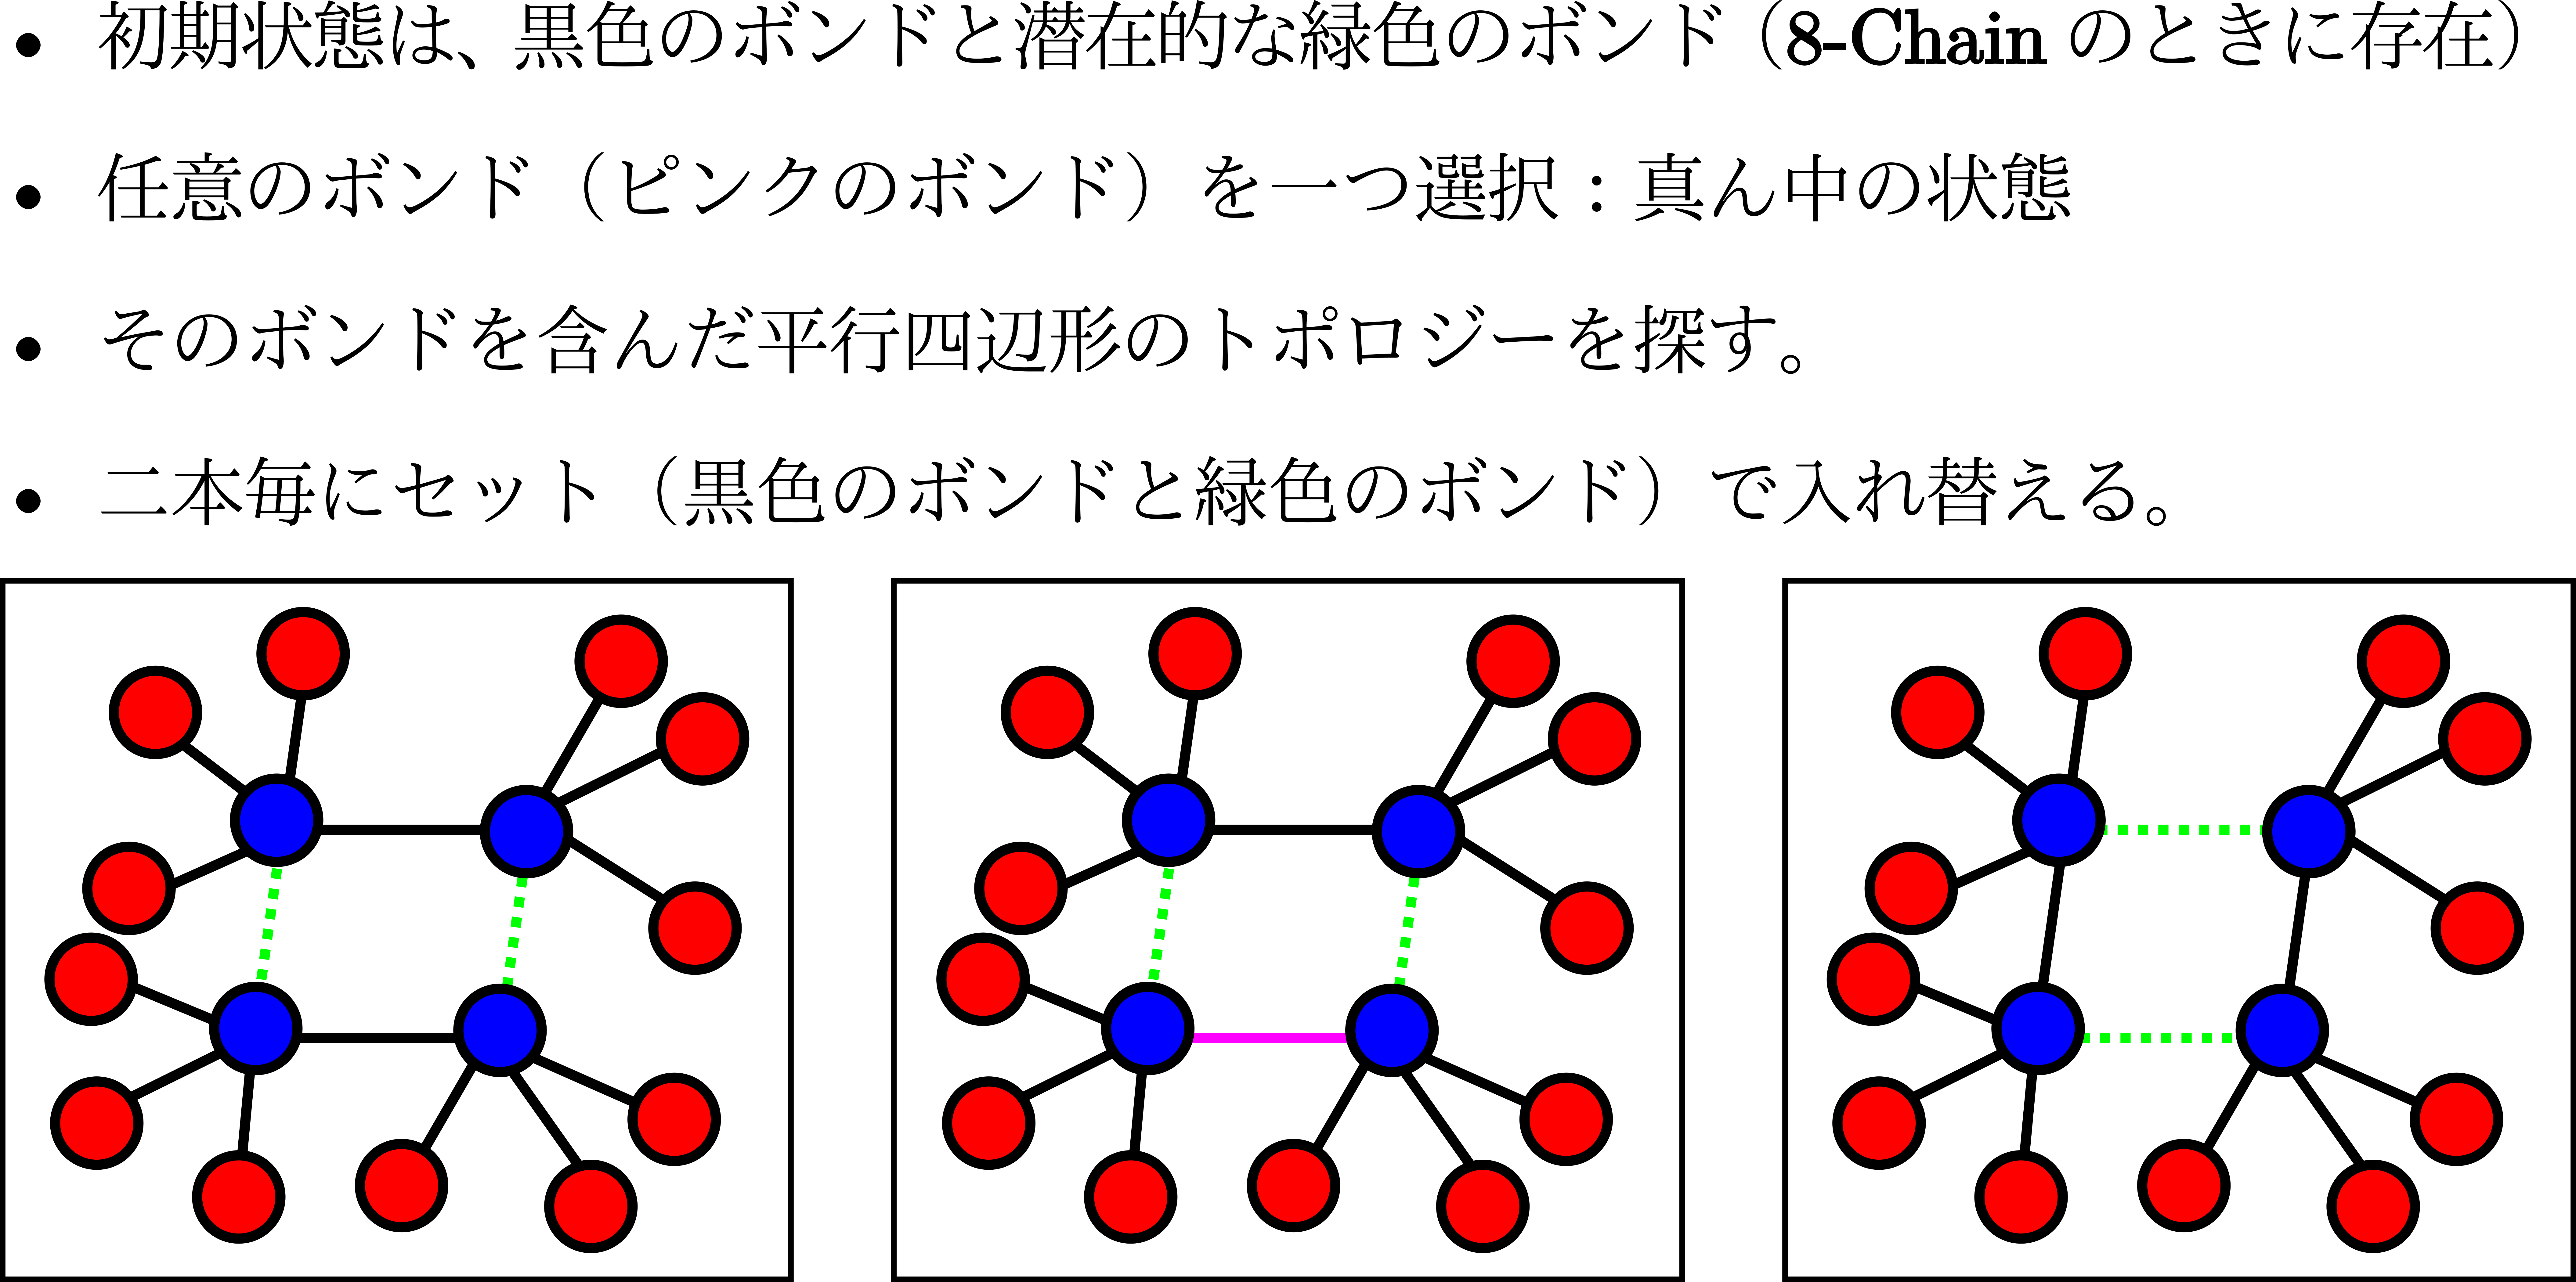
\includegraphics[width=\textwidth]{bond_exchg.png}
\end{columns}